\documentclass{beamer}
\setbeamertemplate{navigation symbols}{}

\usepackage{amsmath}
\usepackage{hyperref}
\usetheme{Montpellier}


\beamersetuncovermixins{\opaqueness<1>{25}}{\opaqueness<2->{15}}
\begin{document}
\title{LU Decomposition}  
\author{By\\ Dilip Puri\\Govind Meena\\Hemant Kumar}
\date{\today} 
\begin{frame}
\titlepage
\end{frame}

%\begin{frame}\frametitle{Table of contents}\tableofcontents
%\end{frame} 

\section{Problem} 
\begin{frame}\frametitle{Problem} 
We have a matrix A, now we want to decompose matrix A into two matrices L(Lower Triangular Matrix) and U(Upper Triangular Matrix) such that \\
\begin{center}
\begin{LARGE}
\textbf{A = L * U}\\
where
\begin{equation*}
L = \left[ \begin{aligned}
1 && 0 && 0 \\
a && 1 && 0 \\
b && c && 1
\end{aligned}
\right]\,,
U = \left[ \begin{aligned}
d && e && f \\
0 && g && h \\
0 && 0 && i
\end{aligned}
\right]\,.
\end{equation*}
\end{LARGE}
\end{center}
\end{frame}


\section{Motivation} 
\begin{frame}\frametitle{Motivation} 
\texttt{So the first question come to mind that why we are doing this?}\\
so straight forward answer would be that it will simplify things. How?\\
Most of the time in mathematics modeling we came up with system of linear equations in the form of\\
\begin{center}
\begin{LARGE}
\textbf{Ax = b}
\end{LARGE}
\end{center}
so finding $A^{-1}$ is quite difficult so we will use LU decomposition\\
\begin{center} \begin{huge}
How?
\end{huge} \end{center}
\end{frame}

\begin{frame}{Example}
Lets we have system of eqations
\begin{align*}
  [A]\{x\} = \{b\}\\
  	[L][U]\{x\} = \{b\}\\
  	(\therefore [A] = [L][U])\\
  \{y\} = [U]\{x\}\\
  [L]\{y\} = \{b\}\\
  \because []=matrix, \{\}=vector
\end{align*}
This will make our system so simple to solve...
\end{frame}

\begin{frame}{Example}
\begin{equation*}
A = \left[ \begin{aligned}
1 && 2 && 4 \\
3 && 8 && 14 \\
2 && 6 && 13
\end{aligned}
\right]\,,
x = \left[ \begin{aligned}
x_1\\
x_2\\
x_3
\end{aligned}
\right]\,,
b = \left[ \begin{aligned}
3\\
13\\
4
\end{aligned}
\right]\,.
\end{equation*}
\begin{equation*}
A= LU \Rightarrow \left[ \begin{aligned}
1 && 0 && 0 \\
a && 1 && 0 \\
b && c && 1
\end{aligned}
\right]\,*
\left[ \begin{aligned}
d && e && f \\
0 && g && h \\
0 && 0 && i
\end{aligned}
\right]\,=
\left[ \begin{aligned}
d && e && f \\
ad && ae+g && af+h \\
bd && be+cg && bf+ch+i
\end{aligned}
\right]\,.
\end{equation*}
\begin{equation*}
\Rightarrow
\left[ \begin{aligned}
d && e && f \\
ad && ae+g && af+h \\
bd && be+cg && bf+ch+i
\end{aligned}
\right]\,=
\left[ \begin{aligned}
1 && 2 && 4 \\
3 && 8 && 14 \\
2 && 6 && 13
\end{aligned}
\right]\,
\end{equation*}
Now compare the values and get the values of elements of L and U.
\end{frame}

\begin{frame}%{Example}
\begin{equation*}
L = \left[ \begin{aligned}
1 && 0 && 0 \\
3 && 1 && 0 \\
2 && 1 && 1
\end{aligned}
\right]\,,
U = \left[ \begin{aligned}
1 && 2 && 4 \\
0 && 2 && 2 \\
0 && 0 && 3
\end{aligned}
\right]\,.
\end{equation*}
The next step is to solve [L]\{y\}=\{b\} for the vector \{y\} that we consider
\begin{equation*}
Ly = \left[ \begin{aligned}
1 && 0 && 0 \\
3 && 1 && 0 \\
2 && 1 && 1
\end{aligned}
\right]\,*
\left[ \begin{aligned}
y_1 \\
y_2 \\
y_3
\end{aligned}
\right]\,=
\left[ \begin{aligned}
3 \\
13 \\
4
\end{aligned}
\right]\,=
b
\end{equation*}
which can be solved by forward substitution \{y\} = [3 4 -6$]^T$ now that we have found y we finish the procedure by solving
\begin{equation*}
Ux = \left[ \begin{aligned}
1 && 2 && 4 \\
0 && 2 && 2 \\
0 && 0 && 3
\end{aligned}
\right]\,*
\left[ \begin{aligned}
x_1 \\
x_2 \\
x_3
\end{aligned}
\right]\,=
\left[ \begin{aligned}
3 \\
4 \\
-6
\end{aligned}
\right]\,=
y
\end{equation*}
by using backward substitution we will get \{x\}.
\end{frame}

\section{Methods}
\begin{frame}{Methods}
There are many methods of LU decompositions like:\\
\hspace*{2cm} Gaussian Elimination\\
\hspace*{2cm} Doolittle's method\\
\hspace*{2cm} Crout's method\\
\hspace*{2cm} and many more...\\
so what are implementing here is: \texttt{Doolittle's method}
\end{frame}
\begin{frame}{Algorithm}
%for j=1:n\\
%\hspace*{1cm}	for i=j:n\\
%\hspace*{1.5cm}	for k=0:i-1\\
%\hspace*{2cm}$L_{ik}U_{kj}$ = $A_{ij}$ gives row i of U\\
%\hspace*{1.5cm}	end\\
%\hspace*{1cm}	end\\
%\hspace*{1cm}	for j=i:n\\
%\hspace*{1.5cm}	for k=0:j-1\\
%\hspace*{2cm}$L_{ik}U_{kj}$ = $A_{ij}$ gives row i of L\\
%\hspace*{1.5cm}	end\\
%\hspace*{1cm}	end\\
%end	
\begin{center}
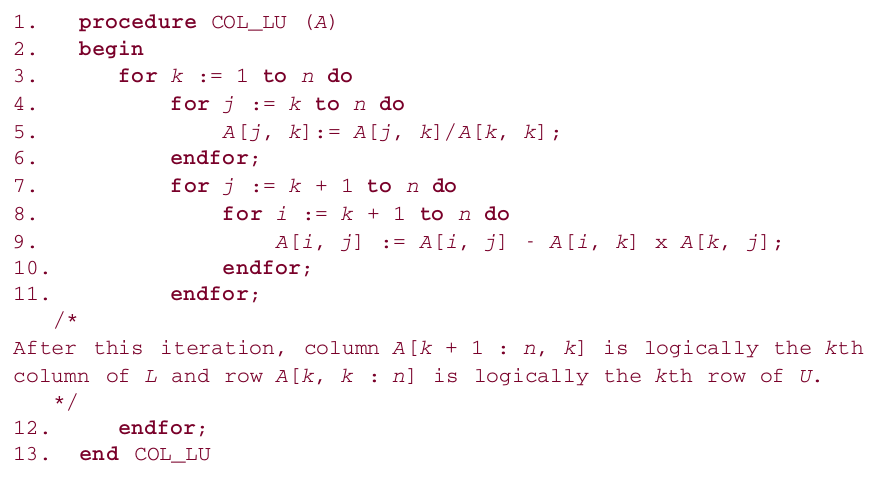
\includegraphics[scale=.28]{algo.png}\\
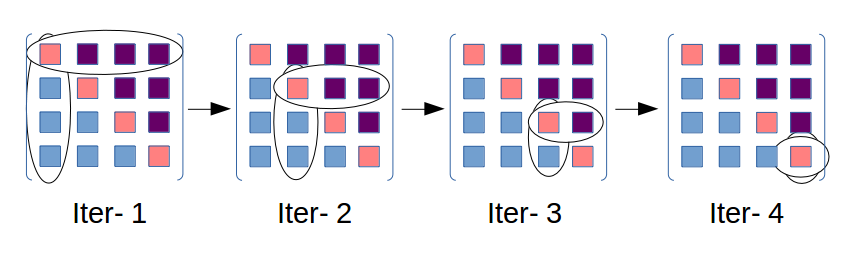
\includegraphics[scale=.3]{pic1.png}
\end{center}
\end{frame}

\section{Tasks}
\begin{frame}{Task Generation and Dependency Graph}
\begin{columns}
\begin{column}{4cm}
\begin{enumerate}
\item $L_{11}$ = $a_{11}$
\item $L_{21}$ = $a_{21}$
\item $L_{31}$ = $a_{31}$
\item $U_{12}$ = $\frac{a_{12}}{L_{11}}$
\item $L_{22}$ = $a_{22} - L_{21}U_{12}$
\item $L_{32}$ = $a_{32} - L_{31}U_{12}$
\item $U_{13}$ = $\frac{a_{13}}{L_{11}}$
\item $U_{23}$ = $\frac{a_{23} - L_{23}U_{13}}{L_{22}}$
\item $L_{33}$ = $a_{33} - L_{31}U_{13} - L_{32}U_{23}$
\end{enumerate}
\end{column}
\begin{column}{7cm}
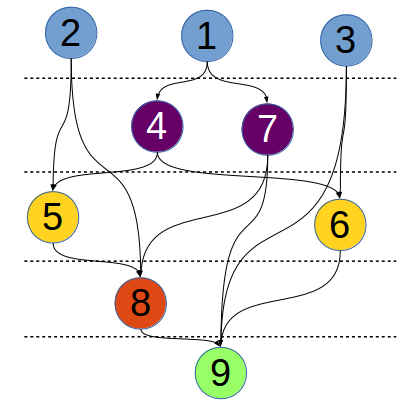
\includegraphics[scale=.5]{taskdep.png}
\end{column}
\end{columns}
\end{frame}

\section{Performance}
\begin{frame}{Time Scalability}
\begin{center}
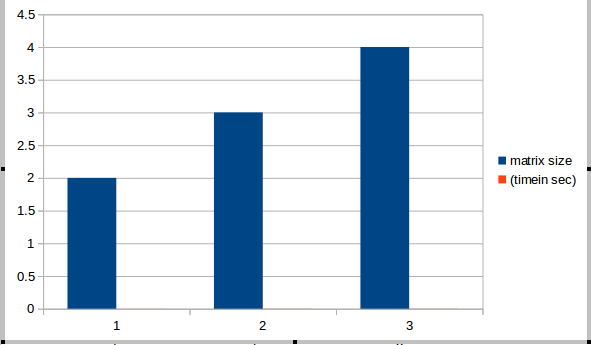
\includegraphics[scale=.4]{grapg.png}
\end{center}
\end{frame}
\begin{frame}{Time Scalability}
\begin{center}
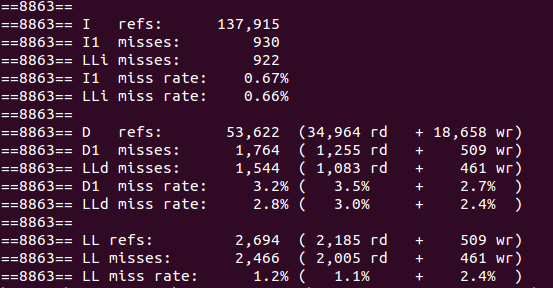
\includegraphics[scale=.4]{l33.png}
\end{center}
\end{frame}
\begin{frame}{Complexity}
Time  = O($n^3$)\\
Space = Two nxn matrices space
\end{frame}

\section{What is Next ??}
\begin{frame}{What is Next ??}
\begin{center}

\includegraphics[scale=.2]{pic3.jpg}
\end{center}
\end{frame}
\begin{frame}
\begin{center}
\begin{huge}
Make Algorithm Parallel\\
\end{huge}
Thank You!\footnote{Resources: wikipedia.orgadf\\http://www.engr.colostate.edu/~thompson/hPage/CourseMat/Tutorials/CompMethods/doolittle.pdf}
\end{center}
\end{frame}

\end{document}